\documentclass{lab_sheet}
\usepackage{hyperref}
\def\ddfrac#1#2{\displaystyle\frac{\displaystyle #1}{\displaystyle #2}}
\begin{document}
\titlePage{Review of Convolution}{January 2, 2022}
\pagenumbering{roman}
\clearpage
\tableofcontents
\clearpage
\phantomsection
\addcontentsline{toc}{section}{\bfseries{List of Figures}}
\listoffigures
\clearpage
\phantomsection
\addcontentsline{toc}{section}{\bfseries{Listings}}
\lstlistoflistings
\clearpage
\pagenumbering{arabic}
\section{Objectives}
\begin{itemize}
\item To be able to perform convolution of two given signal using basic formula.
	\item To be able to perform convolution of two given signals using Python (\texttt{NumPy}) functions.
\end{itemize}
\section{Functions Used}
\begin{itemize}
	\item \texttt{conv}: \texttt{conv} is an in-built Matlab function to find convolution of input arrays.
	\item \texttt{sinc}: \texttt{sinc} is an in-built Matlab function to return the $sinc$ response of the input.
\end{itemize}
\section{Packages Used}
\begin{itemize}
	\item \texttt{NumPy}: \texttt{NumPy} is a fundamental package for scientific computing with Python.
	\item \texttt{Matplotlib}: \texttt{Matplotlib} is a comprehensive library for creating static, animated, and interactive visualizations in Python.
\end{itemize}
\section{Background Theory}
The output of any Linear Time Invariant (LTI) system is some sort of operation between input and system response; the operation is nothing but convolution, denoted by symbol $\circledast$, and defined as,
\begin{equation}
	y(t)=x(t)\circledast h(t)=\int_{-\infty}^{\infty}x(\tau)h(t-\tau)d\tau
	\label{eqn:ct_convo}
\end{equation}

\begin{equation}
	y[n]=x[n]\circledast h[n]=\int_{k=-\infty}^{\infty}x[k]h[n-k]
	\label{eqn:dt_convo}
\end{equation}
Equation~\ref{eqn:ct_convo} is known as convolution integral and is defined for continuous time signals where as Equation~\ref{eqn:dt_convo} is known as convolution sum and is defined for discrete time signals.
\\
For a causal LTI system, the convolution sum is given by,
\begin{equation}
	y[n]=\int_{k=0}^{n}x[k]h[n-k]
	\label{eqn:causal_convo}
\end{equation}
The process of computing the convolution between x[k] and h[k] involves the following four
steps:

\textbf{1. Folding}: Fold $h[k]$ about $k=0$ to obtain $h[-k]$.
\matlabcode{sigfold}{Matlab function for folding}
\textbf{2. Shifting}: Shift $h[-k]$ by $n_0$ to the right (left if $n_o$ is positive (negative), to obtain $h[n_o-k]$.
\matlabcode{sigshift_m}{Matlab function for shifting}
\textbf{3. Multiplication}: Multiply $x[k]$ by $h[n_o–k]$ to obtain the product sequence $V_{n_o}[k]$ where, $V_{n_o}[k]=x[k].h[n_o-k]$.
\matlabcode{sigmulti}{Matlab function for multiplication}
\textbf{4. Summation}: Sum all the values of the product sequence $V_{n_o}$ to obtain the value of
the output at times $n=n_o$.
\newpage
\textbf{Example:} \textit{Convolution of signals $x[n]$ and $h[n]$ by graphical, tabular and} \texttt{conv} \textit{function.}
\matlabcode{example_all}{Matlab script to find convolution of example using graphical, tabular and conv}
\begin{figure}[H]
	\centering
	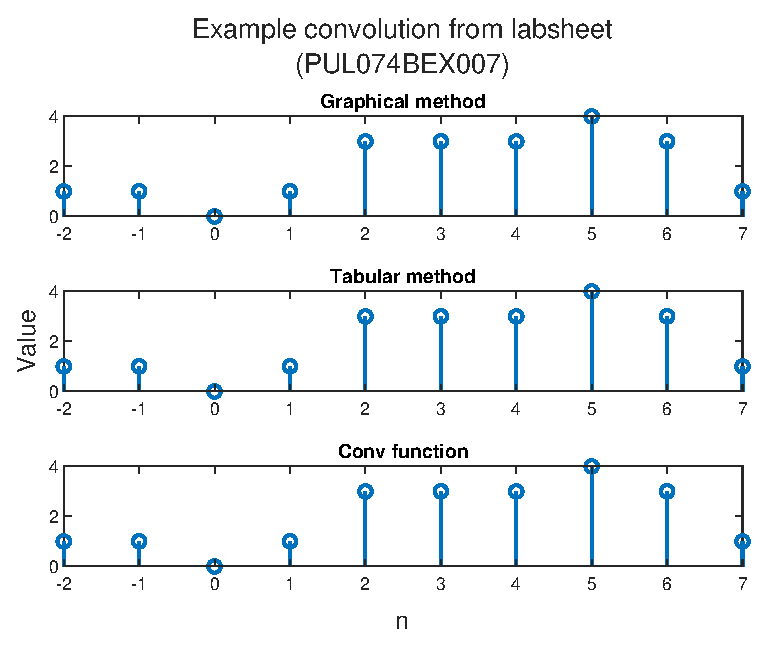
\includegraphics[width=0.8\linewidth]{../Figures/lab_3_example_all.eps}
	\caption{Example convolution using graphical, tabular and conv}
	\label{fig:example}
\end{figure}
\section{Lab Exercises}
\mysub{Convolution using basic convolution formula}
\problem{Find the convolution result of the following signal using basic convolution formula.}
\begin{verbatim}
        X1(n1)=[1,1,1,1,1]
        n1=[-2,-1,0,1,2]
        X2(n2)=[1,0,0,0,0,0,0,0,0,0]
        n2=[-4,-3,-2,-1,0,1,2,3,4,5]
        X2 is a periodic signal.
        Y2=X1*X2
    \end{verbatim}
\matlabcode{lab_3_1}{Matlab script for convolution using basic convolution formula}
\begin{figure}[H]
	\centering
	\includegraphics[width=0.73\linewidth]{../Figures/lab_3_1_ml.eps}
	\caption{Observation of convolution using basic convolution formula (Matlab)}
	\label{fig:3_1_ml}
\end{figure}
\pythoncode{lab_3_1}{Python script for convolution using basic convolution formula}
\begin{figure}[H]
	\centering
	\includegraphics[width=0.8\linewidth]{../Figures/lab_3_1_py.eps}
	\caption{Observation of convolution using basic convolution formula (Python)}
	\label{fig:3_1_py}
\end{figure}
\mysub{Convolution using \texttt{conv} and \texttt{convolve} function}
\problem{Find the convolution using \texttt{conv} and \texttt{convolve} function.
}
\mysubsub{DT convolution}
\subproblem{\begin{equation*}
		x[n]= \begin{cases}
			\ddfrac{1}{3}n \quad \text{for} \quad 0\leq n \leq 6 \\
			0 \quad \text{else}
		\end{cases}
		\quad\text{and,}\quad
		h[n]= \begin{cases}
			1 \quad \text{for} \quad -2\leq n \leq 2 \\
			0 \quad \text{else}
		\end{cases}
	\end{equation*}}
\matlabcode{lab_3_2_a}{Matlab script for DT convolution using conv function}
\begin{figure}[H]
	\centering
	\includegraphics[width=0.73\linewidth]{../Figures/lab_3_2_a_ml.eps}
	\caption{Observation of DT convolution using conv function (Matlab)}
	\label{fig:3_2_a_ml}
\end{figure}
\pythoncode{lab_3_2_a}{Python script for DT convolution using convolve function}
\begin{figure}[H]
	\centering
	\includegraphics[width=0.8\linewidth]{../Figures/lab_3_2_a_py.eps}
	\caption{Observation of DT convolution using convolve function (Python)}
	\label{fig:3_2_a_py}
\end{figure}
\mysubsub{CT convolution}
\subproblem{$$
	x(t)=u(t)\quad \text{and,} \quad
	h(t)=e^{-at}u(t), \text{ where }a>0
$$}
\matlabcode{lab_3_2_b}{Matlab script for CT convolution using conv function}
\begin{figure}[H]
	\centering
	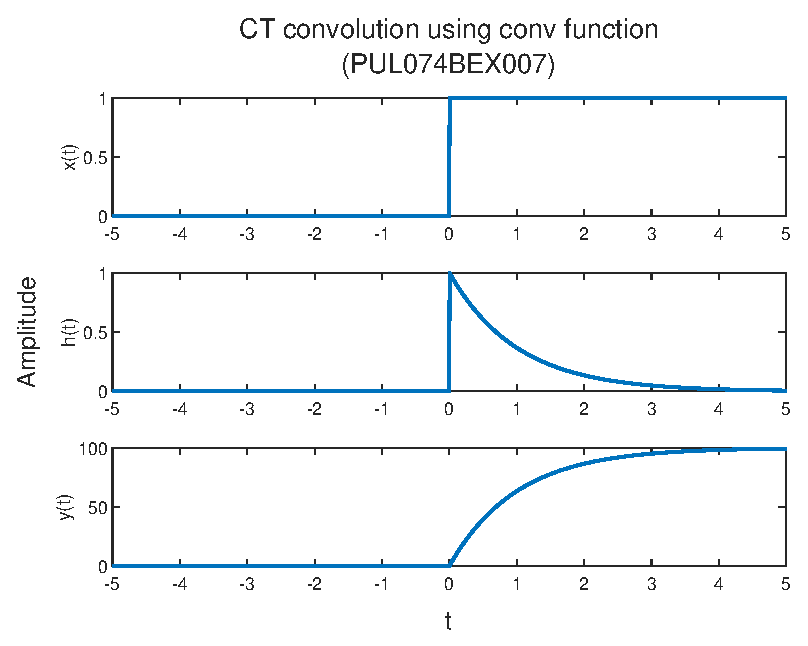
\includegraphics[width=0.73\linewidth]{../Figures/lab_3_2_b_ml.eps}
	\caption{Observation of CT convolution using conv function (Matlab)}
	\label{fig:3_2_b_ml}
\end{figure}
\pythoncode{lab_3_2_b}{Python script for CT convolution using convolve function}
\begin{figure}[H]
	\centering
	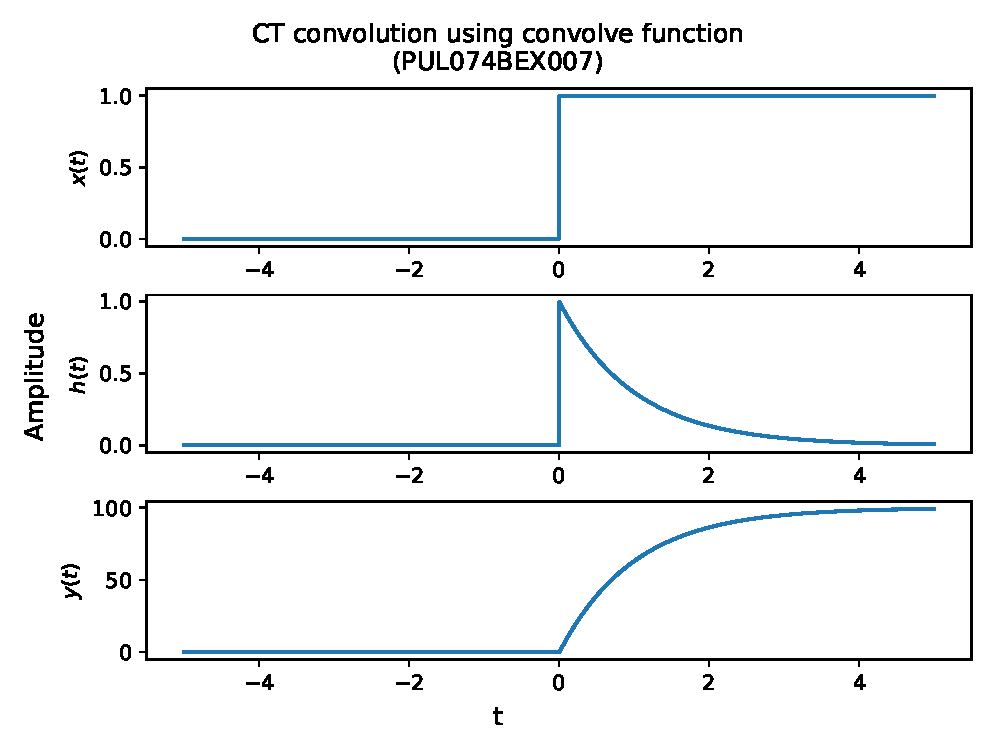
\includegraphics[width=0.8\linewidth]{../Figures/lab_3_2_b_py.eps}
	\caption{Observation of CT convolution using convolve function (Python)}
	\label{fig:3_2_b_py}
\end{figure}
\mysub{LTI system response in DT}
\problem{Consider two discrete time sequences $x[n]$ and $h[n]$ given by
}
\begin{equation*}
	x[n]=\begin{cases}
		1 \quad \textbf{for} \quad 0\leq n \leq 4 \\
		0 \quad \textbf{elsewhere}
	\end{cases}
	\quad \textbf{and,} \quad h[n]=\begin{cases}
		2^n \quad \textbf{for} \quad 0\leq n \leq 6 \\
		0 \quad \textbf{elsewhere}
	\end{cases}
\end{equation*}
\textbf{a. Find the response of the LTI system with impulse response $h[n]$ to input $x[n]$.}\\
\textbf{b. Plot the signals and comment on the result.}
\matlabcode{lab_3_3}{Matlab script for finding response of LTI system}
\begin{figure}[H]
	\centering
	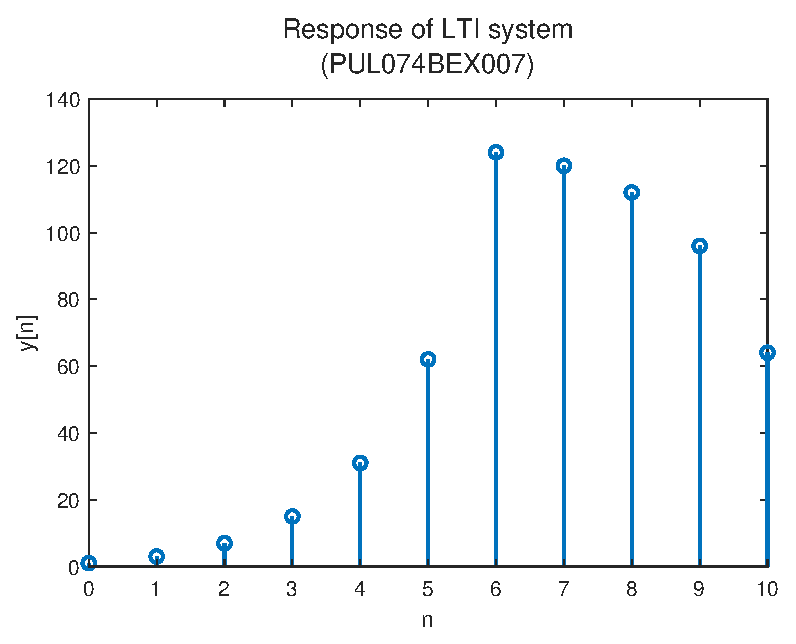
\includegraphics[width=0.73\linewidth]{../Figures/lab_3_3_ml.eps}
	\caption{Observation of response of LTI system (Matlab)}
	\label{fig:3_3_ml}
\end{figure}
\pythoncode{lab_3_3}{Python script for finding response of LTI system}
\begin{figure}[H]
	\centering
	\includegraphics[width=0.8\linewidth]{../Figures/lab_3_3_py.eps}
	\caption{Observation of response of LTI system (Python)}
	\label{fig:3_3_py}
\end{figure}
The output response for the given LTI system goes on increasing up to $n=6$ and then decays for the rest of the observable time.
\mysub{LTI system response in CT with impulse response as \texttt{sinc} functions}
\problem{If the impulse response $h(t)$ of a LTI system is given by \texttt{sinc} function and input signal $x(t)$ is a rectangular wave given as,
$$h(t)=\ddfrac{2\tau}{T_p}sinc\left(\ddfrac{2\tau t}{T_p}\right) \quad \text{and,} \quad x(t)=\begin{cases}
		1 \quad \text{for} \quad 1\leq t \leq 100 \\
		0 \quad \text{elsewhere}
	\end{cases}$$
Find output of the system for different values of $\tau$. Comment on the result.}
\matlabcode{lab_3_4}{Matlab script for finding response of LTI system with sinc function as impulse response}
\begin{figure}[H]
	\centering
	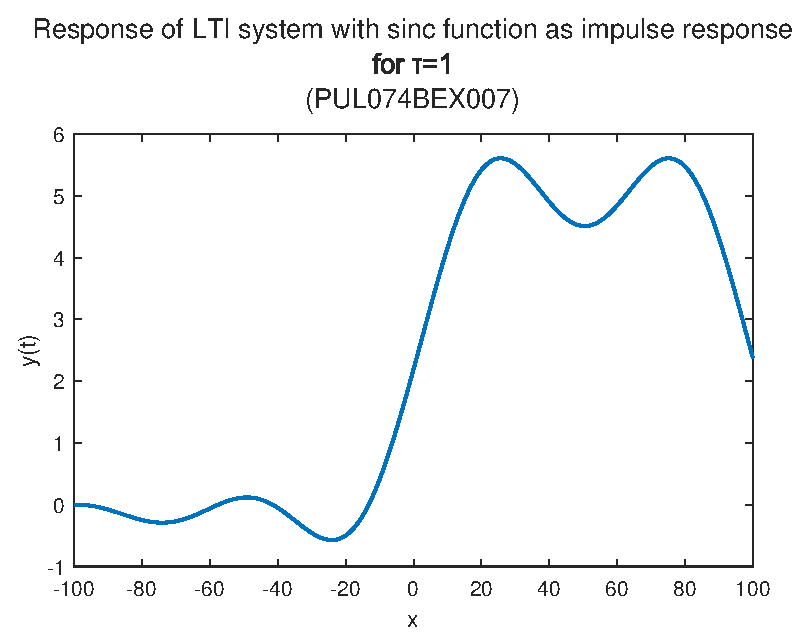
\includegraphics[width=0.73\linewidth]{../Figures/lab_3_4_ml.eps}
	\caption{Observation of response of LTI system with sinc function as impulse response (Matlab)}
	\label{fig:3_4_ml}
\end{figure}
\pythoncode{lab_3_4}{Python script for finding response of LTI system with sinc function as impulse response}
\begin{figure}[H]
	\centering
	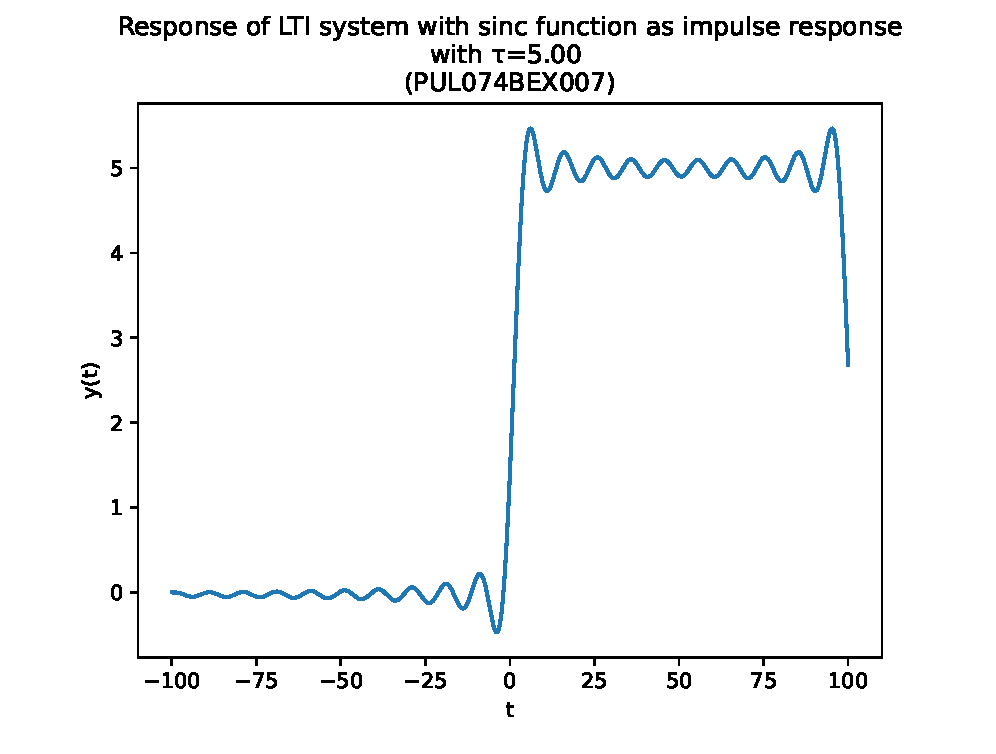
\includegraphics[width=0.8\linewidth]{../Figures/lab_3_4_py.eps}
	\caption{Observation of response of LTI system with sinc function as impulse response (Python)}
	\label{fig:3_4_py}
\end{figure}
The output response for the given LTI system where the impulse response is a sinc function changes with change in the value of $\tau$.
\section{Discussion and Conclusion}
In this lab experiment, we performed convolution using different techniques. Initially, with the example problem in the lab sheet, convolution using graphical, tabular and in-built \texttt{conv} function was visualized in Matlab. Then, we performed convolution with the basic formula in both Matlab and Python. Following that, we performed convolution of DT and CT signals with \texttt{conv} function in Matlab and \texttt{convolve} function in Python using \texttt{NumPy}. The output response of an LTI system in DT was also visualized, which was the convolution sum of the input $x[n]$ and impulse response $h[n]$. Finally, output response of an LTI system in CT with the \texttt{sinc} function as the impulse response was visualized.\\
Hence, the objectives of the lab experiment were fulfilled.
\end{document}